	\chapter{Planteamiento del Problema}
	\section{Descripción de la Realidad Problemática}

	Lima Metropolitana, con una población superior a los 10 millones de habitantes, enfrenta un grave problema de deterioro en sus pavimentos debido al tráfico vehicular intenso y las condiciones climáticas. La falta de un sistema de monitoreo eficiente ha resultado en un elevado costo de mantenimiento y en la proliferación de daños en las vías, como grietas y baches. Estos deterioros, no gestionados de manera adecuada, afectan la movilidad, la seguridad vial y la calidad de vida de los ciudadanos. A pesar de los esfuerzos del Ministerio de Transportes y Comunicaciones (MTC) para destinar fondos al mantenimiento, las intervenciones no son suficientes ni oportunas.  \parencite{ws_oms2022cancert}

	A continuación, se presentan la Figura \ref{1:fig} y la Figura \ref{1:fig2} que muestran los distintos índices de incidencia y mortalidad de cáncer de tiroides en mujeres, donde se puede resaltar la presencia de Perú en los rangos más altos de cada uno de estos. 
	\begin{comment}
	\begin{figure}[H]
		\begin{center}
			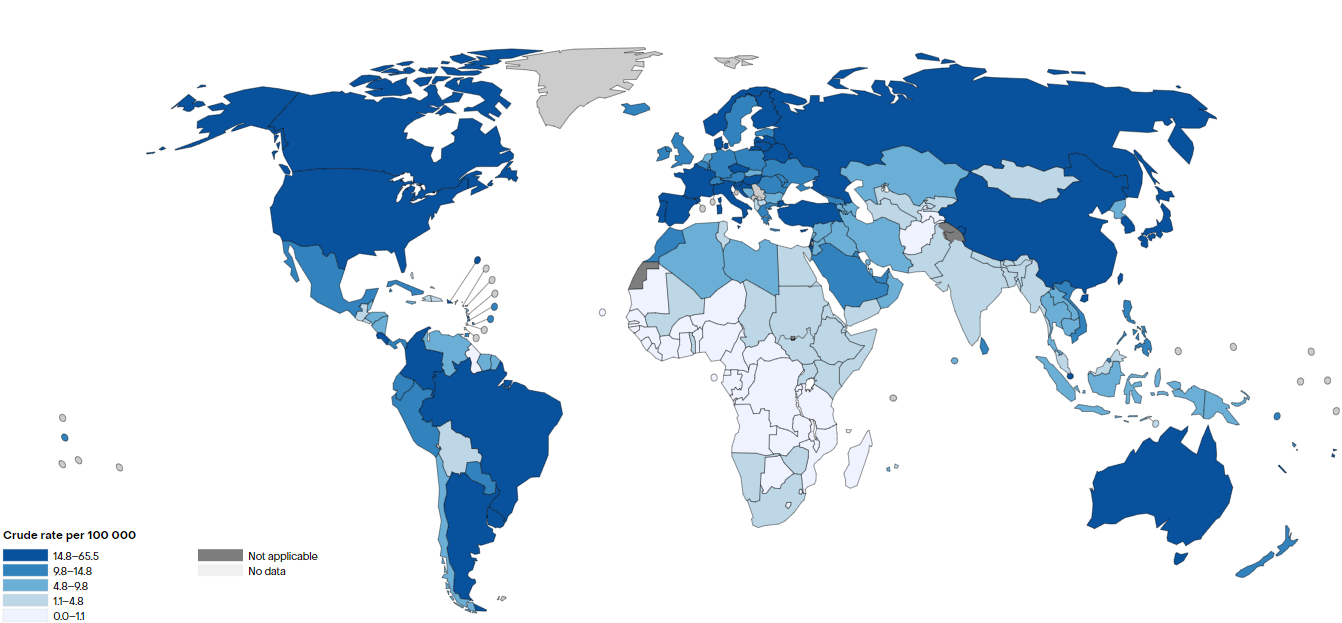
\includegraphics[width=1.00 \textwidth]{1/figures/tb_inc_ct_mujeres.png}
			\caption[Tasa bruta de incidencia de cáncer de tiroides en mujeres por 100 000 personas]{Tasa bruta de incidencia de cáncer de tiroides en mujeres por 100 000 personas. \\
			Fuente: \cite{ws_oms2022cancert}. \textit{Cancer Today}.}
			\label{1:fig}
		\end{center}
	\end{figure}


	\begin{figure}[H]
		\begin{center}
			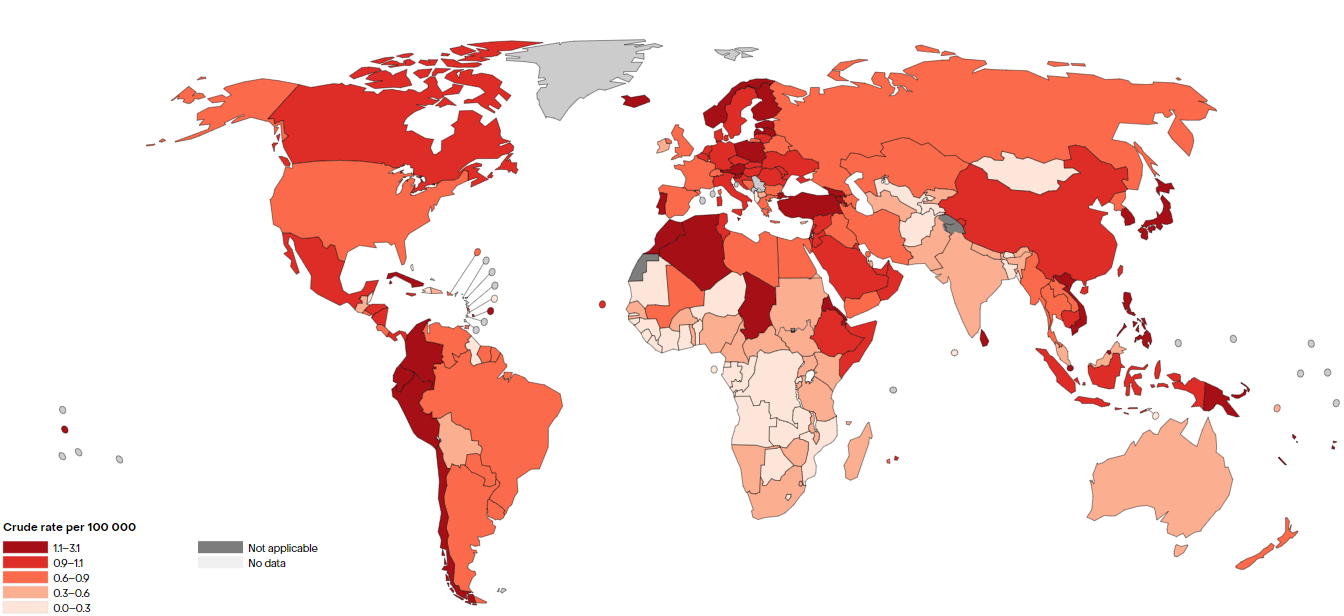
\includegraphics[width=1.00 \textwidth]{1/figures/tb_mor_ct_mujeres.png}
			\caption[Tasa bruta de mortalidad de cáncer de tiroides en mujeres por 100 000 personas]{Tasa bruta de mortalidad de cáncer de tiroides en mujeres por 100 000 personas. \\
			Fuente: \cite{ws_oms2022cancert}. \textit{Cancer Today}.}
			\label{1:fig2}
		\end{center}
	\end{figure}

	De igual forma, en el caso de los varones, el Perú también se encuentra entre los rangos más altos de incidencia y mortalidad. A continuación, se muestran estos datos en la Figura \ref{1:fig3} y Figura \ref{1:fig4}.

	\begin{figure}[H]
		\begin{center}
			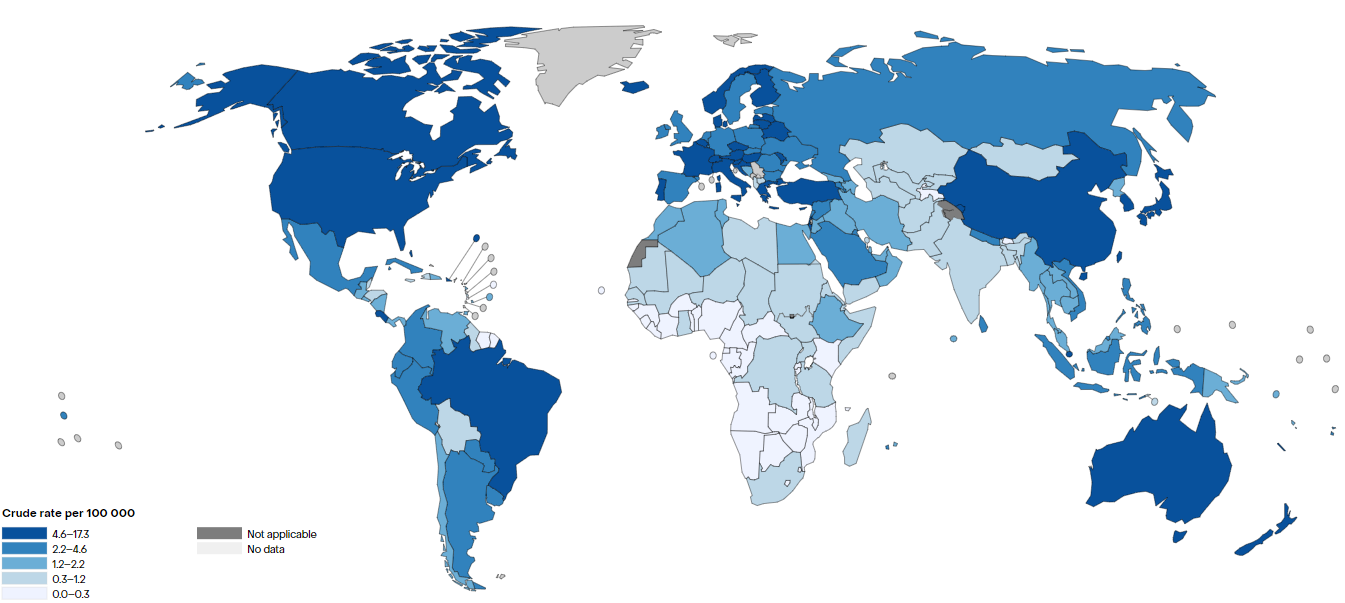
\includegraphics[width=1.00 \textwidth]{1/figures/tb_inc_ct_varones.png}
			\caption[Tasa bruta de incidencia de cáncer de tiroides en varones por 100 000 personas]{Tasa bruta de incidencia de cáncer de tiroides en varones por 100 000 personas. \\
			Fuente: \cite{ws_oms2022cancert}. \textit{Cancer Today}.}
			\label{1:fig3}
		\end{center}
	\end{figure}

	\begin{figure}[H]
		\begin{center}
			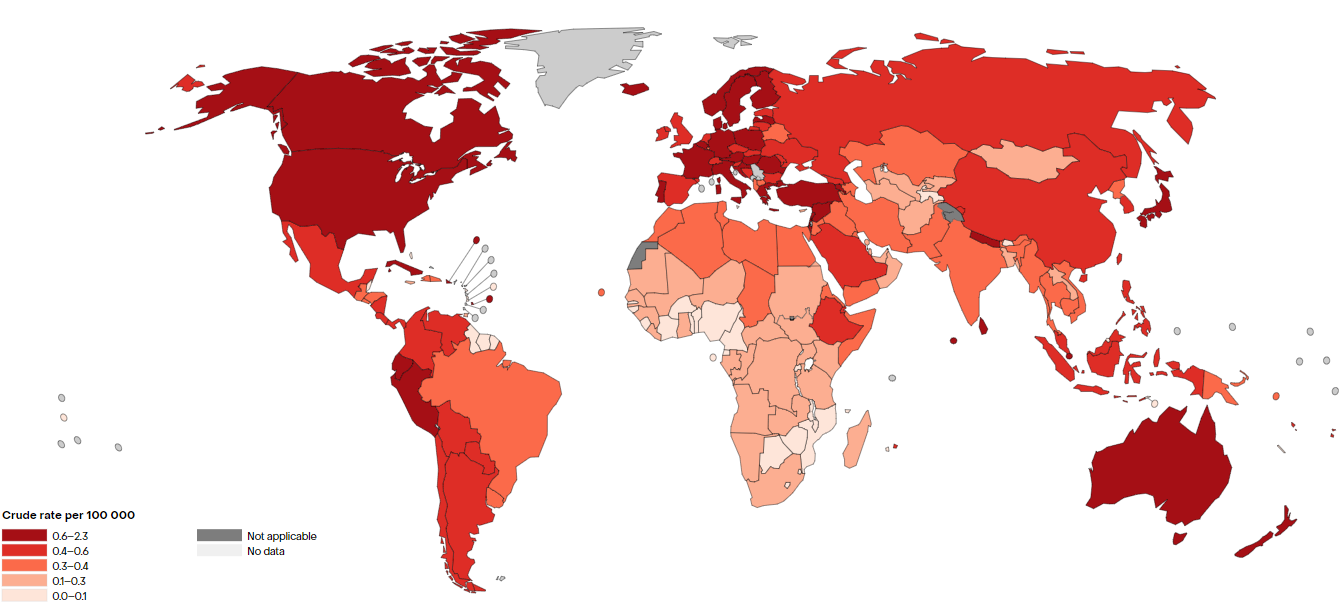
\includegraphics[width=1.00 \textwidth]{1/figures/tb_mor_ct_varones.png}
			\caption[Tasa bruta de mortalidad de cáncer de tiroides en varones por 100 000 personas]{Tasa bruta de mortalidad de cáncer de tiroides en varones por 100 000 personas. \\
			Fuente: \cite{ws_oms2022cancert}. \textit{Cancer Today}.}
			\label{1:fig4}
		\end{center}
	\end{figure}

	Con la Figura \ref{1:fig5} que muestra los mismos índices distribuidos por género y regiones del mundo, es fácil notar la alta incidencia de este tipo de cáncer en las mujeres, siendo la región con mayor incidencia América del Norte, mientras que la de mayor mortalidad es Oceanía. La región de Latino América y el Caribe supera a Norte América en mortalidad, aunque se encuentra por debajo de Oceanía y Europa.

	\begin{figure}[H]
		\begin{center}
			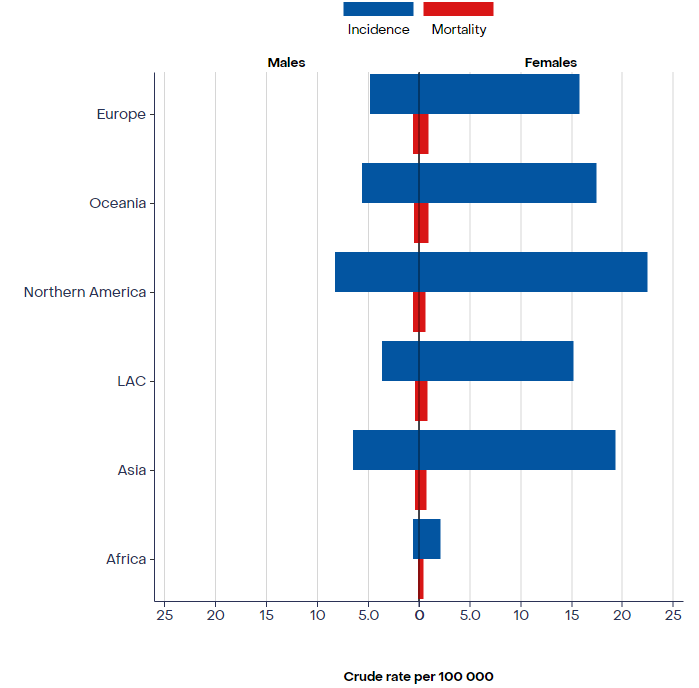
\includegraphics[width=0.60 \textwidth]{1/figures/tb_inc_mor_gen_y_reg.png}
			\caption[Tasa bruta de incidencia y mortalidad de cáncer de tiroides por género y región]{Tasa bruta de incidencia y mortalidad de cáncer de tiroides por género y región. \\
			Fuente: \cite{ws_oms2022cancert}. \textit{Cancer Today}.}
			\label{1:fig5}
		\end{center}
	\end{figure}
	\end{comment}
	El avance de la inteligencia artificial (IA) y la visión por computadora ofrecen la posibilidad de desarrollar sistemas de monitoreo automatizados que puedan detectar daños en tiempo real, optimizando el mantenimiento de las carreteras y disminuyendo los costos asociados a la rehabilitación vial.\parencite{pr_haugen2016amethy}.

	%Para la detección temprana de este tipo de cáncer o desarrollo de tumores, depende en gran medida de la experiencia y la capacidad cognitiva de un experto en radiología, y muchos de estos se ven en la necesidad de utilizar no muy avanzados sistemas de pre-diagnóstico por computadora, mejor conocido como CAD por sus siglas en inglés \parencite{pr_zhu2021agendlframew}. Ante grandes limitaciones de sistemas CAD básicos, y aprovechando el extenso uso de la Inteligencia Artificial, el Deep Learning y sus algoritmos son capaces de incorporar mayor eficacia a dichos sistemas.

	%El Deep Learning ha sido usado ampliamente como herramienta para el procesamiento de imágenes médicas, no solo para detectar diferentes tipos de cáncer o nódulos como los relacionados a los pulmones, sino también para la retinopatía diabética y localización de feto en ecografías, e inclusive en la detección del COVID-19 \parencite{pr_bhatta2021medimage}. Además, el aumento de la calidad de imágenes de ultrasonido que se fue desarrollando en los últimos 30 años, aumentando cada vez más resolución de las imágenes y reduciendo el tiempo de adquisición, ha permitido una mejora en términos de detección de enfermedad; sin embargo, aún se requiere de un médico especializado y debidamente entrenado para lograr un realizar un correcto análisis de las imágenes, por ello se vio en la necesidad de encontrar métodos de clasificación automatizada, pero dichos métodos antiguos consumían bastante tiempo, gran poder computacional y poca capacidad de generalización de resultados, es así que en este contexto, apareció una novedosa arquitectura de Deep Learning que actualmente es usado en diferentes áreas el día de hoy: las Redes Neuronales Convolucionales o CNN, quitando en gran medida los problemas de las antigua técnicas \parencite{pr_signgh20203ddl}. Sin embargo, es importante mencionar que estos últimos años han ido apareciendo nuevas arquitecturas capaces incluso de superar a los ya altamente difundidos CNN. Y es que a pesar del dominio actual de estas redes, las arquitecturas basadas en Transformer han ido tomando cada vez más mayor importancia dentro del mundo de la Inteligencia Artificial, y esto incluye también el área de procesamiento de imágenes médicas gracias a los Vision Transformers o ViT, una versión de los Transformers originales orientados al procesamiento de imágenes.
	
	%El desarrollo de estas nuevas tecnologías basadas en distintos algoritmos de Inteligencia Artificial, ya sea en CNN, ViT o incluso ambos, podrían mejorar aún más los tiempos de pre-diagnóstico de nódulos tiroideos y, además, aumentar los porcentajes de aciertos de los especialistas en estas tareas de diagnóstico a través de un trabajo conjunto con estas tecnologías de alto potencial.



	\section{Formulación del Problema}
	Con el objetivo de formular los objetivos de esta investigación, se propusieron las siguientes preguntas.
	\subsection{Problema General}
	PG: \newcommand{\ProblemaGeneral}{
	¿Cómo se podría detectar y gestionar de manera automatizada y eficiente el desgaste y deterioro de los pavimentos en Lima Metropolitana para reducir los costos de mantenimiento y mejorar la seguridad vial?
	}
	\ProblemaGeneral
	\subsection{Problemas Específicos}
	\newcommand{\Pbone}{
	¿Cómo podría implementarse un sistema automatizado para monitorear y clasificar en tiempo real el deterioro de los pavimentos?
	}
	\newcommand{\Pbtwo}{
	¿De qué manera podría reducirse el costo económico derivado de la rehabilitación tardía de carreteras en mal estado?
	}
	\newcommand{\Pbthree}{
	¿Cómo se podría minimizar el riesgo de accidentes de tránsito ocasionados por el mal estado de las vías urbanas?
	}
	\newcommand{\Pbfour}{
	¿Qué estrategias permitirían priorizar la reparación de las áreas más deterioradas para optimizar la distribución de los recursos?
	}

	\begin{itemize}
		\item PE1: {\Pbone}
		\item PE2: {\Pbtwo}
		\item PE3: {\Pbthree}
		\item PE4: {\Pbfour}
	\end{itemize}

	\section{Objetivos de la Investigación}
	A continuación, se presentan el objetivo general y los objetivos específicos.
	\subsection{Objetivo General}
	OG: \newcommand{\ObjetivoGeneral}{
	Desarrollar un modelo de clasificación automatizada utilizando redes neuronales convolucionales (CNN) para detectar y clasificar el deterioro de los pavimentos en Lima Metropolitana, optimizando el mantenimiento y mejorando la seguridad vial.
	}
	\ObjetivoGeneral
	\subsection{Objetivos Específicos}
	\newcommand{\Objone}{
	Implementar un sistema de monitoreo y clasificación basado en IA y visión por computadora para la identificación de grietas y baches en tiempo real.
	}
	\newcommand{\Objtwo}{
	Analizar el impacto económico de la detección temprana de daños en la infraestructura vial de Lima.
	}
	\newcommand{\Objthree}{
	Priorizar áreas críticas de deterioro para optimizar el uso de los recursos en las intervenciones de mantenimiento.
	}
	\newcommand{\Objfour}{
	Evaluar la precisión y eficiencia del modelo propuesto frente a métodos tradicionales de inspección vial.
	}

	\begin{itemize}
		\item OE1: {\Objone}
		\item OE2: {\Objtwo}
		\item OE3: {\Objthree}
		\item OE4: {\Objfour}
	\end{itemize}

	\section{Hipótesis}
	
	\subsection{Hipótesis General}
	La implementación de un modelo automatizado de clasificación de deterioros en pavimentos, basado en redes neuronales convolucionales, mejorará la detección y el mantenimiento de las vías en Lima Metropolitana, reduciendo costos y aumentando la seguridad vial.
	\subsection{Hipótesis Específicos}

	\newcommand{\Hione}{
	El uso de redes neuronales convolucionales permitirá una clasificación más precisa del estado de los pavimentos respecto a métodos tradicionales.}
	\newcommand{\Hitwo}{
	La detección automatizada y en tiempo real reducirá el tiempo de respuesta para las reparaciones, minimizando los costos a largo plazo.}
	\newcommand{\Hithree}{
	La priorización de las zonas más deterioradas mejorará la eficiencia en la asignación de recursos.}
	

	\begin{itemize}
		\item H1: {\Hione}
		\item H2: {\Hitwo}
		\item H3: {\Hithree}
	\end{itemize}


	\section{Justificación de la Investigación}

	\subsection{Teórica}
	La investigación aportará al campo de la inteligencia artificial aplicada a la infraestructura urbana, ampliando el conocimiento sobre el uso de redes neuronales convolucionales para la clasificación de imágenes en un contexto de mantenimiento vial.
	\subsection{Práctica}
	La implementación del sistema propuesto contribuirá a mejorar la gestión del mantenimiento de carreteras en Lima Metropolitana, reduciendo los costos asociados a reparaciones y mejorando la seguridad de los ciudadanos.
	\subsection{Metodológica}
	El estudio aplicará metodologías de redes neuronales convolucionales y técnicas de visión por computadora, lo que permitirá validar la efectividad de modelos de IA para tareas de clasificación en escenarios reales de infraestructura vial.
	\section{Delimitación del Estudio}
	A continuación, se presentará la delimitación espacial, temporal y conceptual.

	\subsection{Espacial}
	El estudio se llevará a cabo en las principales vías urbanas de Lima Metropolitana, donde se concentra el mayor flujo vehicular y deterioro de pavimentos.
	\subsection{Temporal}
	La investigación se desarrollará durante el período de 2024, con recolección de datos de campo y pruebas en un entorno controlado para evaluar el rendimiento del modelo propuesto.
	\subsection{Conceptual}
	El estudio se centrará en la aplicación de redes neuronales convolucionales para la clasificación de imágenes de pavimentos en estado de deterioro, considerando las variables clave de desgaste, como grietas y baches.